\documentclass[conference]{IEEEtran}
\IEEEoverridecommandlockouts
\usepackage{cite}
\usepackage{amsmath,amssymb,amsfonts}
\usepackage{algorithmic}
\usepackage{graphicx}
\usepackage{textcomp}
\usepackage{xcolor}
\usepackage{listings}
\usepackage[bookmarks=true,breaklinks=true,letterpaper=true,colorlinks,linkcolor=black,citecolor=blue,urlcolor=black]{hyperref}

% dsm: Copied from /usr/share/texlive/texmf-dist/tex/latex/listings/lstlang1.sty ,
% but removing bin from morekeywords[2], b/c deletekeywords ignores it somehow.
\lstdefinelanguage{PythonNoBin}%
  {morekeywords={access,and,break,class,continue,def,del,elif,else,%
      except,exec,finally,for,from,global,if,import,in,is,lambda,not,%
      or,pass,print,raise,return,try,while},%
  % Built-ins
   morekeywords=[2]{abs,all,any,basestring,bool,bytearray,callable,chr,
     classmethod,cmp,compile,complex,delattr,dict,dir,divmod,enumerate,eval,
     execfile,file,filter,float,format,frozenset,getattr,globals,hasattr,
     help,hex,id,input,int,isinstance,issubclass,iter,len,list,locals,long,map,
     max,memoryview,min,object,oct,open,ord,pow,property,range,raw_input,
     reduce,reload,repr,reversed,round,set,setattr,slice,sorted,staticmethod,str,
     sum,super,tuple,type,unichr,unicode,vars,xrange,zip,apply,buffer,coerce,
     intern},
   sensitive=true,%
   morecomment=[l]\#,%
   morestring=[b]',%
   morestring=[b]",%
   morestring=[s]{'''}{'''},% used for documentation text (mulitiline strings)
   morestring=[s]{"""}{"""},% added by Philipp Matthias Hahn
   morestring=[s]{r'}{'},% `raw' strings
   morestring=[s]{r"}{"},%
   morestring=[s]{r'''}{'''},%
   morestring=[s]{r"""}{"""},%
   morestring=[s]{u'}{'},% unicode strings
   morestring=[s]{u"}{"},%
   morestring=[s]{u'''}{'''},%
   morestring=[s]{u"""}{"""}%
  }%

  \lstdefinestyle{custompython}{
 %aboveskip=0in,
 belowskip=0in,
 %abovecaptionskip=0in,
 belowcaptionskip=-10pt,
 %belowcaptionskip=1\baselineskip,
 breaklines=true,
 captionpos=b,
 language=PythonNoBin,
 showstringspaces=false,
 numbers=left,
 stepnumber=1,
 % dsm: semibold
 % yyf: semibold will just be bold on Ubuntu 20.04, disable it
 %basicstyle={\linespread{0.75}\fontseries{sb}\small\ttfamily},
 basicstyle={\linespread{0.75}\footnotesize\ttfamily},
 keywordstyle=\bfseries,
 %% columns=fullflexible,
 xleftmargin=2em,
 frame=single,
 framexleftmargin=2em,
 commentstyle=\itshape\color{green!40!black},
 morekeywords={to,yield,parallel},
}


%\def\BibTeX{{\rm B\kern-.05em{\sc i\kern-.025em b}\kern-.08em
%    T\kern-.1667em\lower.7ex\hbox{E}\kern-.125emX}}
\begin{document}

\title{Optimizing Tensor Product using Sparsity}

\author{\IEEEauthorblockN{Jaeyeon Won}
\and
\IEEEauthorblockN{Ryan Lee}
\and
\IEEEauthorblockN{Nicholas Dow}
}

\maketitle

\begin{abstract}
We present an optimized GPU implementation of the tensor product for equivariant neural networks. Tensor products in equivariant neural networks are challenging due to the block sparsity in its weights imposed by the three properties of equivariance (translation, rotations, and inversion). We show that using the right sparse tensor format is critical to performing only the effectual computations while minimizing costly synchronization between SMs. We implement a GPU implementation using Triton which outperforms the dense Jax-based baseline by XXX$\times$ on a Nvidia RTX A4000 GPU.

\end{abstract}

\section{Introduction}
\label{sec:intro}


Equivariant neural networks\cite{e3nn} are specially designed networks capable of handling input transformations such as rotations and shifts. For instance, if the input to an equivariant neural network is rotated by 90 degrees, the output feature map will transform (or permute) in the same way.

Among the libraries available for building equivariant neural networks, \emph{e3nn-jax}\cite{e3nnjax} stands out as a state-of-the-art tool. It is designed for constructing and accelerating neural networks that are equivariant to 3D rotations, translations, and other symmetries. At its core, e3nn-jax leverages irreducible representations of the 3D rotation group (SO(3)) to process geometric data, such as atomic structures, molecules, and point clouds, within the Jax\cite{jax} framework.

A fundamental operation in e3nn-jax is the tensor product, which combines features expressed in these irreducible representations. This operation enables the network to exchange information between different rotational symmetries while preserving equivariance, ensuring that the model maintains consistency under transformations.


\section{Background}
\label{sec:background}

\subsection{Tensor Product}

In \textbf{e3nn}, there are multiple variants of the tensor product operation. In this project, we focus on a specific form of the tensor product, which can be expressed using Einsum notation as follows:

\[
Out_{b,k} = W_{i,j,k} \ast In1_{b,i} \ast In2_{b,j}
\]

This operation multiplies two batched inputs, \textbf{In1} and \textbf{In2}, with a 3D weight tensor \textbf{W}. The result is stored in \textbf{Out} by reducing over dimensions \(i\) and \(j\).

\subsection{e3nn-jax Implementation}

The current state-of-the-art implementation in e3nn-jax takes advantage of the fact that the weight tensor \(W\) exhibits a special sparsity pattern: a block-diagonal sparse structure. Instead of storing the full tensor \(W_{i,j,k}\), \textbf{e3nn-jax} stores only the dense blocks within \(W\). For each block, the output is computed as:

\[
Out_{b,k} = WBlock_{i,j,k} \ast In1_{b,i} \ast In2_{b,j}
\]

These computations leverage optimized vendor libraries such as cuBLAS\cite{nvidia2021cublas} for efficiency. Additionally, all JAX code is \textit{JIT-compiled}, which significantly accelerates performance compared to running the same code in the Python interpreter.

\subsection{Leveraging Sparsity Limitations}

Despite these optimizations, our investigation revealed that e3nn-jax does not fully exploit the sparsity in \(W\). Specifically, we observed that each dense block within the block-diagonal sparse format has only about \textbf{10\% non-zero values}, meaning a significant number of unnecessary operations (e.g., zero multiplications) are still being performed.

To address this issue, our work implements two optimized versions of the tensor product that fully leverage sparsity and GPU capabilities, reducing redundant computations and improving performance.

\section{Implementation}
\label{sec:impl}

\subsection{Using Coordinate List (COO) Representation}
\label{sec:impl:coo}

The relatively high sparsity of equivariant neural networks guides us to use a \textit{sparse representation} of the weights. Sparse representations such as Coordinate List (COO) and Compressed-Sparse Row only store non-zero values and their coordinates,
which brings the benefit of skipping ineffectual computation (e.g., multiplying by zero). We use the COO format which stores the coordinates of non-zero values as a list of tuples.

%\begin{figure}[!htb]
\begin{lstlisting}[caption={Hash table lookup code.}, label={lst:simple_tensor_prod}, style=custompython]
# B : Batch size
# NNZ: Number of nonzeros
# W_i, W_j, W_k, W_val: weights in COO-format,  dimensions [NNZ]
# Input1, Input2: [B, L_in]
# Output: [B, L_out]
def TensorProduct(W_i, W_j, W_k, W_val, 
  Input1, Input2, Output):
    for nz in range(NNZ):
      nz_in1 = Input1[:,W_i[nz]]
      nz_in2 = Input2[:,W_j[nz]]
      Output[:,W_k[nz]] += nz_in1 * nz_in2 * W_val[nz]
\end{lstlisting}
%\end{figure}

The tensor product kernel is implemented using Triton~\cite{b1}.
We design the kernel such that each Triton program works on a \textit{block of non-zeros}.
The pseudocode is given in \autoref{lst:simple_tensor_prod}.
Given the input \texttt{i}, \texttt{j}, and \texttt{k} coordinate values of the COO,
each Triton program loads a block of these coordinates,
performs an indirect load on the input tensors to grab the corresponding values
(\texttt{i} coordinates from the first tensor and \texttt{j} coordinates from the second tensor),
and multiplies them with the weight.
The kernel then performs scatter indirect stores to the \texttt{k} coordinates
of the output tensor.

Our tensor kernel's performance is highly dependent on the number of gather loads of the input tensors
and the scatter writes to the output tensor.
In particular, the scatter writes must be performed \textit{atomically} because different triton programs (i.e., thread blocks in CUDA-land) can write to the same coordinate of the output tensor.
As we will see later in \autoref{sec:eval}, the atomic add operations dominate our throughput such that the naive implementation is worse than the dense baseline.

\subsection{Reducing Atomic Operations}
\label{sec:impl:block}

We reduce the number of atomic operations by \textit{grouping multiple input coordinates that contribute to the same output coordinate}.
Our key insight is that multiple input coordinates that contribute to the same output coordinate can be handled by a single thread,
which removes the need for atomic operations on those FMAs.

\begin{figure}
  \centering
  \includegraphics[width=1.0\linewidth]{grouped_coo.pdf}
  \caption{Transforming COO to a grouped COO representation with a group size of 2.}
  \label{fig:grouped_coo}
\end{figure}

An example of such grouping is shown in \autoref{fig:grouped_coo}.
We define a new parameter called a \textit{group size} which indicates how many input coordinates are grouped together for the same output coordinate.
Notice that the ideal group size varies per output coordinate,
as the number of input coordinate pairs that have the same output coordinate differ.
To make this amenable to GPUs,
we choose a single group size for all output coordinates and \textit{pad} the input coordinates'
values with zeros if they are not divisible by the group size.
For example, \autoref{fig:grouped_coo} shows that output coordinate 8 only has one input coordinate for it,
so we pad it to match the group size of 2.

%\begin{figure}[!htb]
\begin{lstlisting}[caption={Hash table lookup code.}, label={lst:improved_tensor_prod}, style=custompython]
# B : Batch size
# G_NNZ: Number of grouped output coordinates
# G: group size
# W_i, W_j, W_val: [G_NNZ, G]
# W_k: [G_NNZ]
# Input1, Input2: [B, L_in]
# Output: [B, L_out]
def TensorProduct(W_i, W_j, W_k, W_val, 
  Input1, Input2, Output):
    for nz in range(G_NNZ):
      for g in range(G)
        nz_in1 = Input1[:,W_i[nz, g]]
        nz_in2 = Input2[:,W_j[nz, g]]
        accum += nz_in1 * nz_in2 * W_val[nz, g]
      Output[:,W_k[nz]] += accum
\end{lstlisting}
%\end{figure}

The pseudocode for our improved tensor product kernel is shown in \autoref{lst:improved_tensor_prod}. Each program now loads a block of groups, where each group contains the input coordinate pairs for a given output coordinate. Because each thread now works on a single group, it can accumulate the results across that group locally before storing it back to global memory.

Because grouping introduces padded values, it increases ineffectual computation: compared to the naive implementation which performed $2NNZ \times B$ floating-point multiplies,
grouping now performs $2G\_NNZ \times G \times B$ multiplies where $G\_NNZ >= NNZ$.
The increase in work is determined by the distribution of non-zeros in the weight matrix.
As we will show in the evaluation (\autoref{sec:eval})
we sweep the group size parameter that produces the fastest runtime for our application.



\section{Evaluation}
\label{sec:eval}

We evaluated our implementation on a Nvidia RTX A4000 GPU, with randomly initialized inputs that follow the sparsity pattern 
expected in a real \textbf{e3nn} applications; the sparsity is generated using  \textbf{e3nn's} \texttt{e3nn.clebsch\_gordon} function
who's computation is opaque but generates the weight tensor for the tensor product. We benchmarked both the Naive COO and Padded COO's performances
against the baseline to show the effectiveness of each of the improvments. The parameters that are relevant to check performance against are
the group size parameter (denoted as Padding size), the size of the batch dimension, and the lmax parameter, which controls the number of 
non-zeroes and size of \textbf{In1, In2, and W}. While lmax changes a number of different qualities of the tensor product, the main
one we are concerned with is sparsity.

\begin{figure}[h]
    \centering
    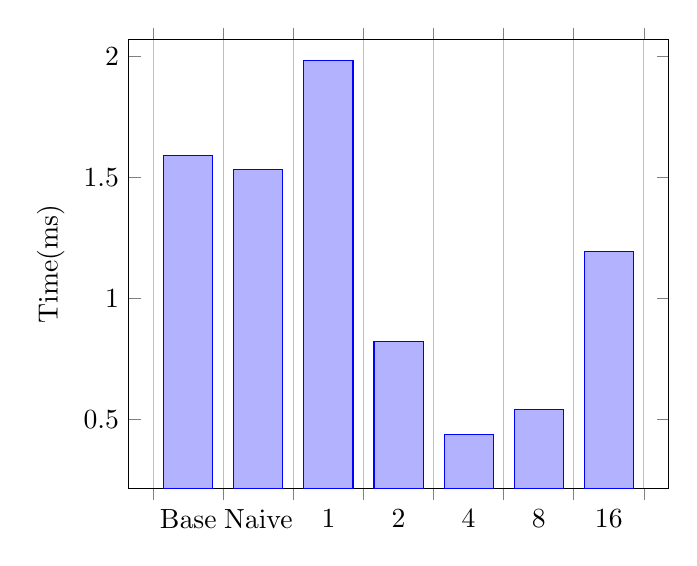
\begin{tikzpicture}
        \begin{axis}[
            ylabel=Time(ms),
            enlargelimits=0.05,
            legend style={at={(0.5,-0.1)},
            anchor=north,legend columns=-1},
            ybar interval=0.7,
            bar width=10pt,
            symbolic x coords={Base, Naive, 1,2,4,8,16, 17},
            xtick=data,
            ymin=.3
        ]
        \addplot % padded COO data
        coordinates {(Base, 1.59) (Naive, 1.534)(1,1.986) (2,0.822)
            (4,0.438) (8,0.542) (16, 1.196) (17, 1.196)};
        \end{axis}
    \end{tikzpicture}
    \caption{Evaluation over padding sizes, Batch size = 1e4, Lmax = 5}
    \label{fig:eval1}
\end{figure}
\subsection{Finetuning group size}
\label{sec:eval:group}
As seen in \autoref{fig:eval1} the group size parameter has a huge impact on the performance of the padded COO implementation. We've found
that performance across batch sizes for a certain group size was independent, but as lmax changed, the optimal group size would change as well.
This observation makes sense intuitively as changing lmax changes the number and distribution of non-zero entries in \textbf{W}, so a group size setting 
for a high lmax might add too many padding zeroes to compute compared to the contention it reduces in the tensor product. However, for all relevant lmax settings(1-5) had group size $\in [3, 5]$.
\begin{figure}
    \centering
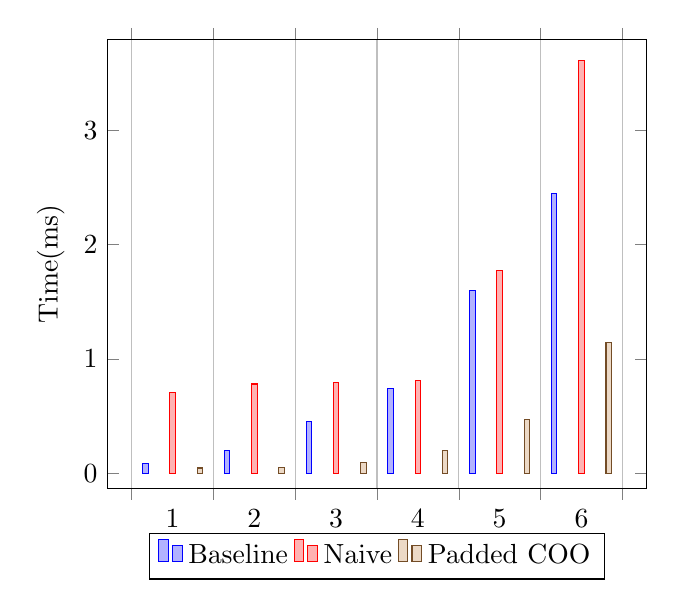
\begin{tikzpicture}
    \begin{axis}[
        x tick label style={
		/pgf/number format/1000 sep=},
        ylabel=Time(ms),
        enlargelimits=0.05,
        legend style={at={(0.5,-0.1)},
        anchor=north,legend columns=-1},
        ybar interval=0.2,
        bar width=1pt,
        symbolic x coords={1,2,3,4,5,6,7},
        xtick=data,
        ymin=.05,
    ]
    \addplot % padded COO data
    coordinates {(1, 0.089) (2, 0.199) (3, 0.457) (4, 0.742) (5, 1.6) (6, 2.451)(7,1)};
    \addplot % padded COO data
    coordinates {(1, 0.711) (2, 0.782) (3, 0.792) (4, 0.815) (5, 1.773) (6, 3.614) (7,1)};
    \addplot % padded COO data
    coordinates {(1, 0.047) (2, 0.05) (3, 0.096) (4, 0.201) (5, 0.472) (6, 1.148) (7,1)};
    \legend{Baseline, Naive, Padded COO}
    \end{axis}
\end{tikzpicture}
\label{fig:eval2}
\caption{Evaluation over Lmax, (Batch size = 1e4, Padding = 4)}
\end{figure}
\subsection{Impact of Lmax on performance}
\label{sec:eval:lmax}
As seen in \autoref{fig:eval2} we can see that Padded COO performs a factor of 4 times better than the baseline and Naive COO for all relevant lmax settings (1-5),
but baseline starts to catch up as lmax grows, with only a 2.5x speedup at lmax = 6. While the sparsity of the tensor product grows as lmax grows and therefore
the theorectical advantage of an implementation leveraged for that sparsity, it seems there are other factors at play limiting that advantage for this 
tensor product.

Combining that observation with the earlier observation that the group size does not change much with different lmax settings, we theorized
that while the sparsity increases with lmax, the distribution of non-zeroes migth be becoming adversarial to our padding approach. With some rudimentary analysis,
we saw that the distribution of non-zeroes per $k$ coordinate was skewed to the left but still maintained outliers at the max value, which increases with lmax.
Perhaps this skew is re-introducing the atomic add contention for some values of $k$ that were previously reduced by grouping, while also increasing the amount
of padding we need to add.

\begin{figure}
    \centering
    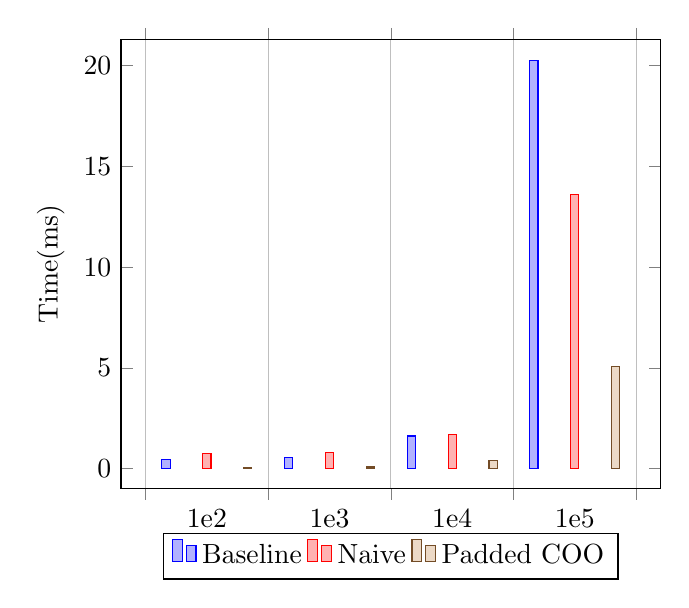
\begin{tikzpicture}
        \begin{axis}[
            x tick label style={
            /pgf/number format/1000 sep=},
            ylabel=Time(ms),
            enlargelimits=0.05,
            legend style={at={(0.5,-0.1)},
            anchor=north,legend columns=-1},
            ybar interval=0.2,
            bar width=1pt,
            symbolic x coords={1e2, 1e3, 1e4, 1e5, 7},
            xtick=data,
            ymin=.05
        ]
        \addplot % padded COO data
        coordinates {(1e2, 0.462) (1e3, 0.562) (1e4, 1.621) (1e5, 20.274) (7,1)};
        \addplot % padded COO data
        coordinates {(1e2, 0.762) (1e3, 0.782) (1e4, 1.711) (1e5, 13.628) (7,1)};
        \addplot % padded COO data
        coordinates {(1e2, 0.045) (1e3, 0.083) (1e4, 0.428) (1e5, 5.082) (7,1)};
        \legend{Baseline, Naive, Padded COO}
        \end{axis}
    \end{tikzpicture}
    \caption{Evaluation over Batch size, (Padding = 4, Lmax = 5)}
    \label{fig:eval3}   
\end{figure}
\subsection{Impact of batch size on performance}
As seen in \autoref{fig:eval3}, Padded COO performs at least a factor of 4 times better than the 
baseline and Naive COO for all batch sizes we could test, but had a bigger advantage at smaller batch sizes before 
speedup plateaued.
\section{Discussion} 
With our project, we successfully leveraged the structured sparsity within the \textbf{e3nn} tensor product to increase
the performance of the tensor product by 2-10x(4-10x for relevant parameters). We also showed that the performance of the
 padded COO implementation is independent of the batch size and group size settings. We also identified a potential scaling problem
 with our approach that would limit speedup on higher values of lmax. 
\subsection{Related Work}
For the tensor product itself, to the best of our knowledge the \textbf{e3nn-jax} tensor product is the state-of-the-art implementation, and 
there are no other public efforts to boost it's performance using it's intrinsic sparsity. While we ended up using Triton as our implementation 
of choice, we unsuccessfully attempted a lower level implementation using NVIDIA's cuSPARSE library\cite{nvidia_cusparse}; the many dimensions of the einsum and converting 
some of the necessary functions to prepare the benchmark from \textbf{e3nn} was too difficult compared to focusing our efforts on Triton.




    

%%%%%%%%% -- BIB STYLE AND FILE -- %%%%%%%%
\bibliographystyle{IEEEtranS}
\bibliography{refs,confs}
%%%%%%%%%%%%%%%%%%%%%%%%%%%%%%%%%%%%
%\begin{thebibliography}{00}
%\bibitem{b1} Tillet, Philippe, Hsiang-Tsung Kung, and David Cox. "Triton: an intermediate language and compiler for tiled neural network computations." Proceedings of the 3rd ACM SIGPLAN International Workshop on Machine Learning and Programming Languages. 2019.
%\end{thebibliography}
%\vspace{12pt}
\end{document}

